% ~~~~~~~~~~~~~~~~~~~~~~~~~~~~~~~~~~~~~~~~~~~~~~~~~~~~~~~~~~~~~~~~~~~~~~~~~~~~~
%                                 RESULTS
% ~~~~~~~~~~~~~~~~~~~~~~~~~~~~~~~~~~~~~~~~~~~~~~~~~~~~~~~~~~~~~~~~~~~~~~~~~~~~~
\chapter{Results}\label{chap:5}
  \lhead{Chapter 5. \emph{Results}}
Our agent is based on multilayer perceptron with one hidden layer consisting of 1000 neurons.
As an activation function we have used logistic sigmoid for hidden layer and linear function
for output layer. Learning rate was set to \(/alpha=0.001\). In our experiments we let both
heuristic players to play against each other and had neural network to observe one of them.
For each state desired output was action executed by heuristic player.

Each plot shows relationship between number of observed actions and success rate against player.
All games were set to maximum 1000 actions -- upon crossing this limit, we consider this as a loss.

\section{ANN vs Random player}

To test whether our agent is learning anything at all, we let him played against pure random
player that selects among all actions with uniform probability. This is of course not meaningful
opponent, but it can tell us how many epochs are required to master this opponent.

We can see that agent was able to learn reasonably fast with less than \(10^7\) observed actions.
Agent does not wins against random all times, because it tends to get stucked in dead end and moving
there back and forth.

\begin{figure}[h!]
  \centering
    \graphicspath{{pictures/}}
  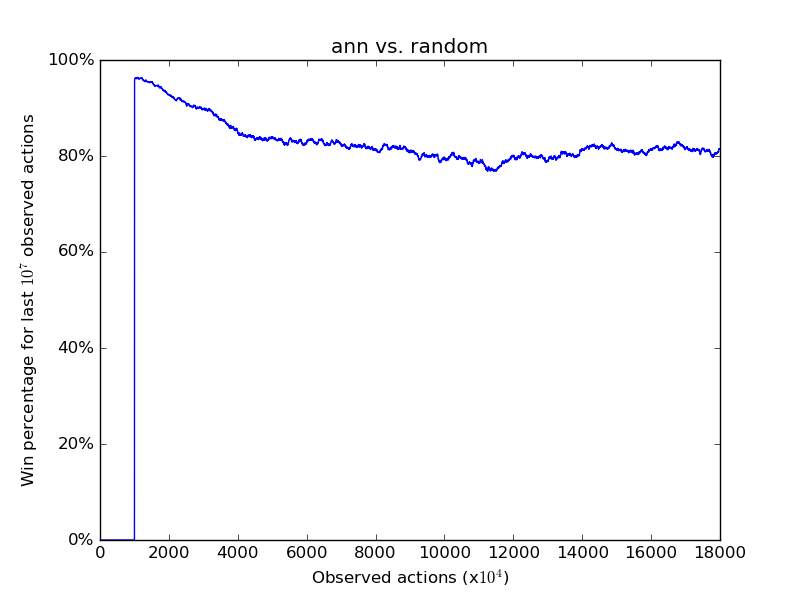
\includegraphics[width=0.50\textwidth]{eps_vs_random.png}
  \vspace*{-0.20cm}
  \caption{ANN vs random player}
  \label{fig:p1}
  \vspace*{-0.00cm}
\end{figure}
\newpage

\section{ANN vs Path player}

In this experiment we let play our agent against player that follows shortest path without ever
placing wall. We can see agent was able to master the game and win every time. Tendency of getting
stucked in dead end did not occur in this scenario because after some number of epochs all games became
100\% deterministic, there was no random.

\begin{figure}[!tbh]
  \centering
    \graphicspath{{pictures/}}
  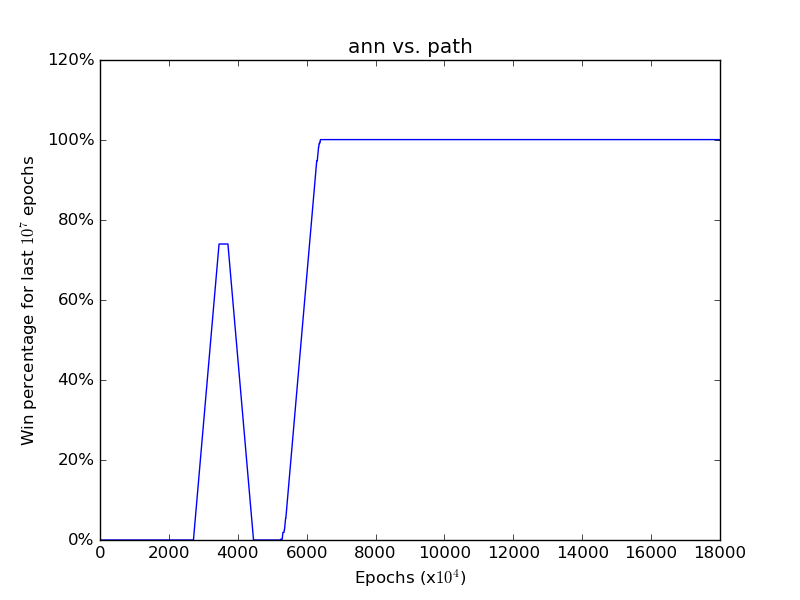
\includegraphics[width=0.50\textwidth]{eps_vs_path.png}
  \vspace*{-0.20cm}
  \caption{ANN vs path player}
  \label{fig:p1}
  \vspace*{-0.00cm}
\end{figure}

\section{ANN vs Heuristic player}

In this last experiment we let play our agent against heuristic player. This was most challenging
task for agent, but we can see tendency of learning was clearly still increasing, although was far
from perfect.

\begin{figure}[t!]
  \centering
    \graphicspath{{pictures/}}
  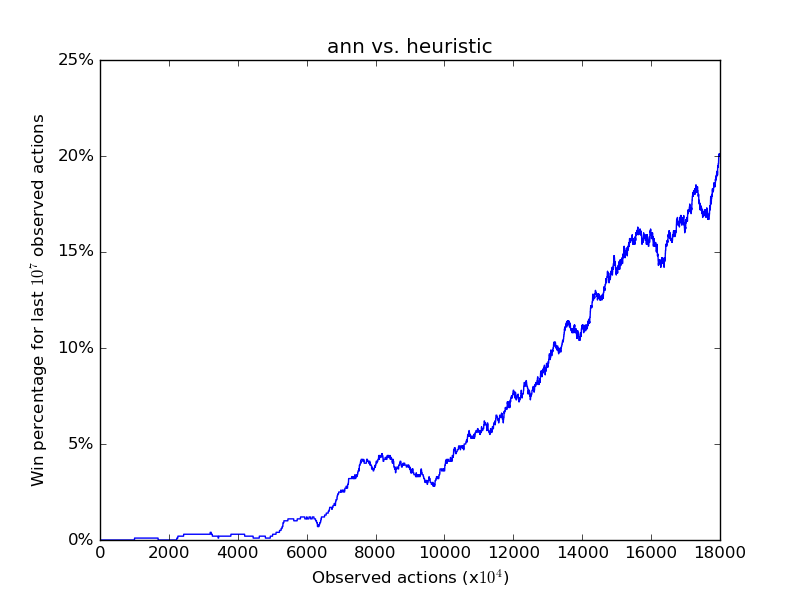
\includegraphics[width=0.50\textwidth]{eps_vs_heuristic.png}
  \vspace*{-0.20cm}
  \caption{ANN vs heuristic player}
  \label{fig:p1}
  \vspace*{-0.00cm}
\end{figure}
